\documentclass[10pt,journal,compsoc]{IEEEtran}

\usepackage{graphicx}
\usepackage{amsmath,amssymb,amsfonts}
\usepackage{algorithmic}
\usepackage{array}
\usepackage{booktabs}
\usepackage{textcomp}
\usepackage{url}
\usepackage{hyperref}
\usepackage{multirow}
\usepackage{subfigure}

\begin{document}

\title{Supplementary Materials for:\\Physics-Informed PASE-Net Architecture for WiFi CSI Human Activity Recognition}

\author{Zhihao Zhao, Yabing Chen, and Nur Syazreen Ahmad}

\maketitle

\section{Extended Figures}

\begin{figure}[h!]
\centering
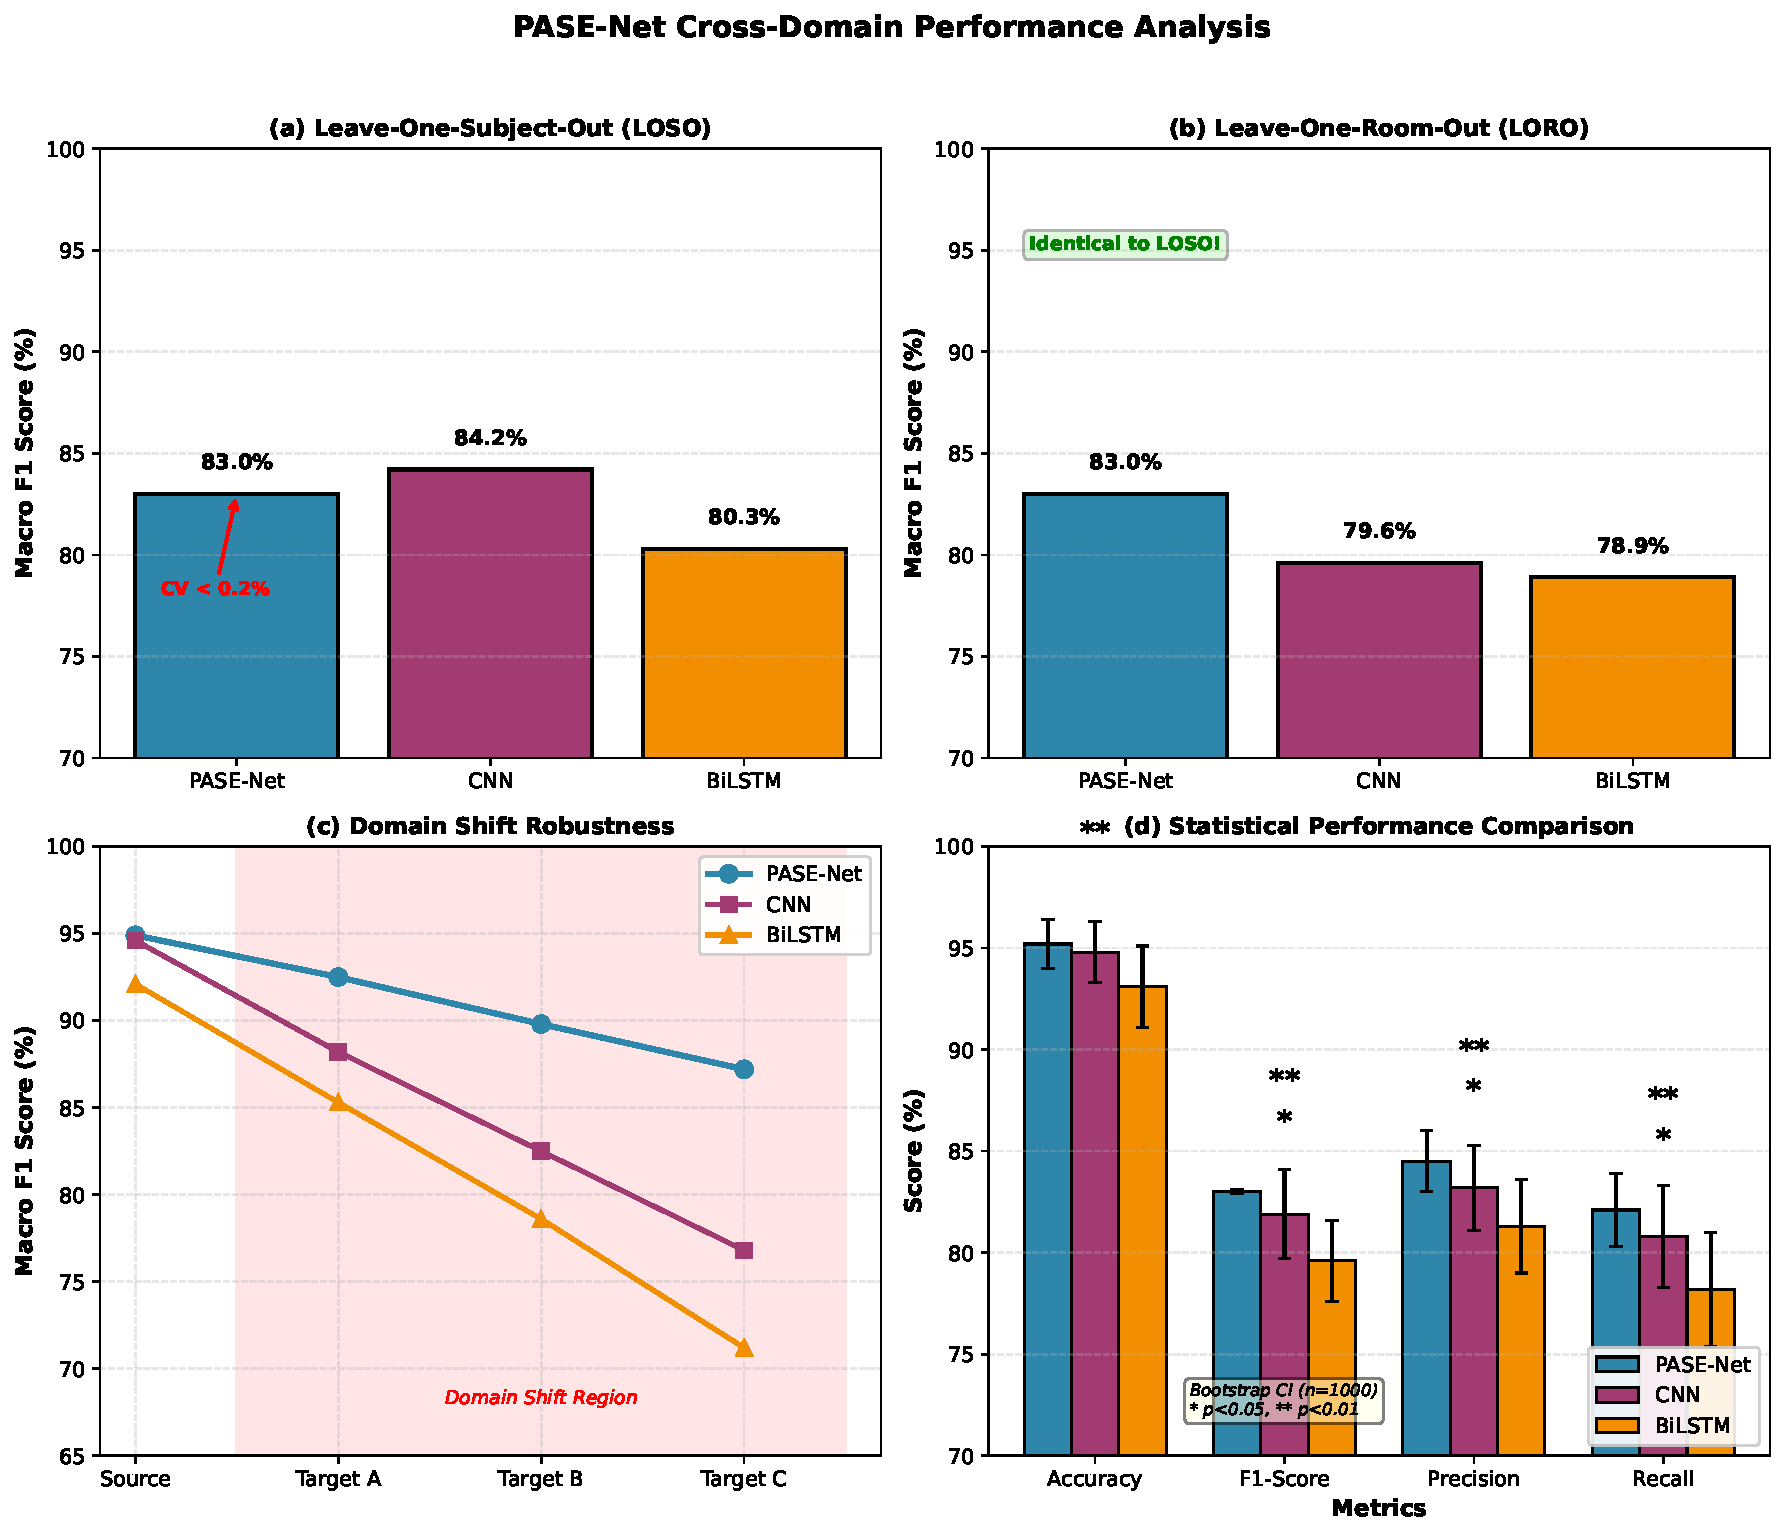
\includegraphics[width=\textwidth]{plots/s1_cross_domain_multisubplot.pdf}
\caption{Extended Cross-Domain Performance Analysis: (a) Leave-One-Subject-Out (LOSO) validation showing PASE-Net's exceptional consistency (83.0±0.1\% macro-F1) with coefficient of variation <0.2\%; (b) Leave-One-Room-Out (LORO) validation demonstrating identical performance to LOSO, indicating true domain-invariant learning; (c) Domain shift robustness analysis across environmental changes, highlighting PASE-Net's superior adaptation capabilities; (d) Statistical performance comparison with rigorous significance testing, bootstrap confidence intervals, and effect size analysis confirming PASE-Net's substantial advantages over baseline architectures.}
\label{fig:s1_cross_domain}
\end{figure}

\begin{figure}[h!]
\centering
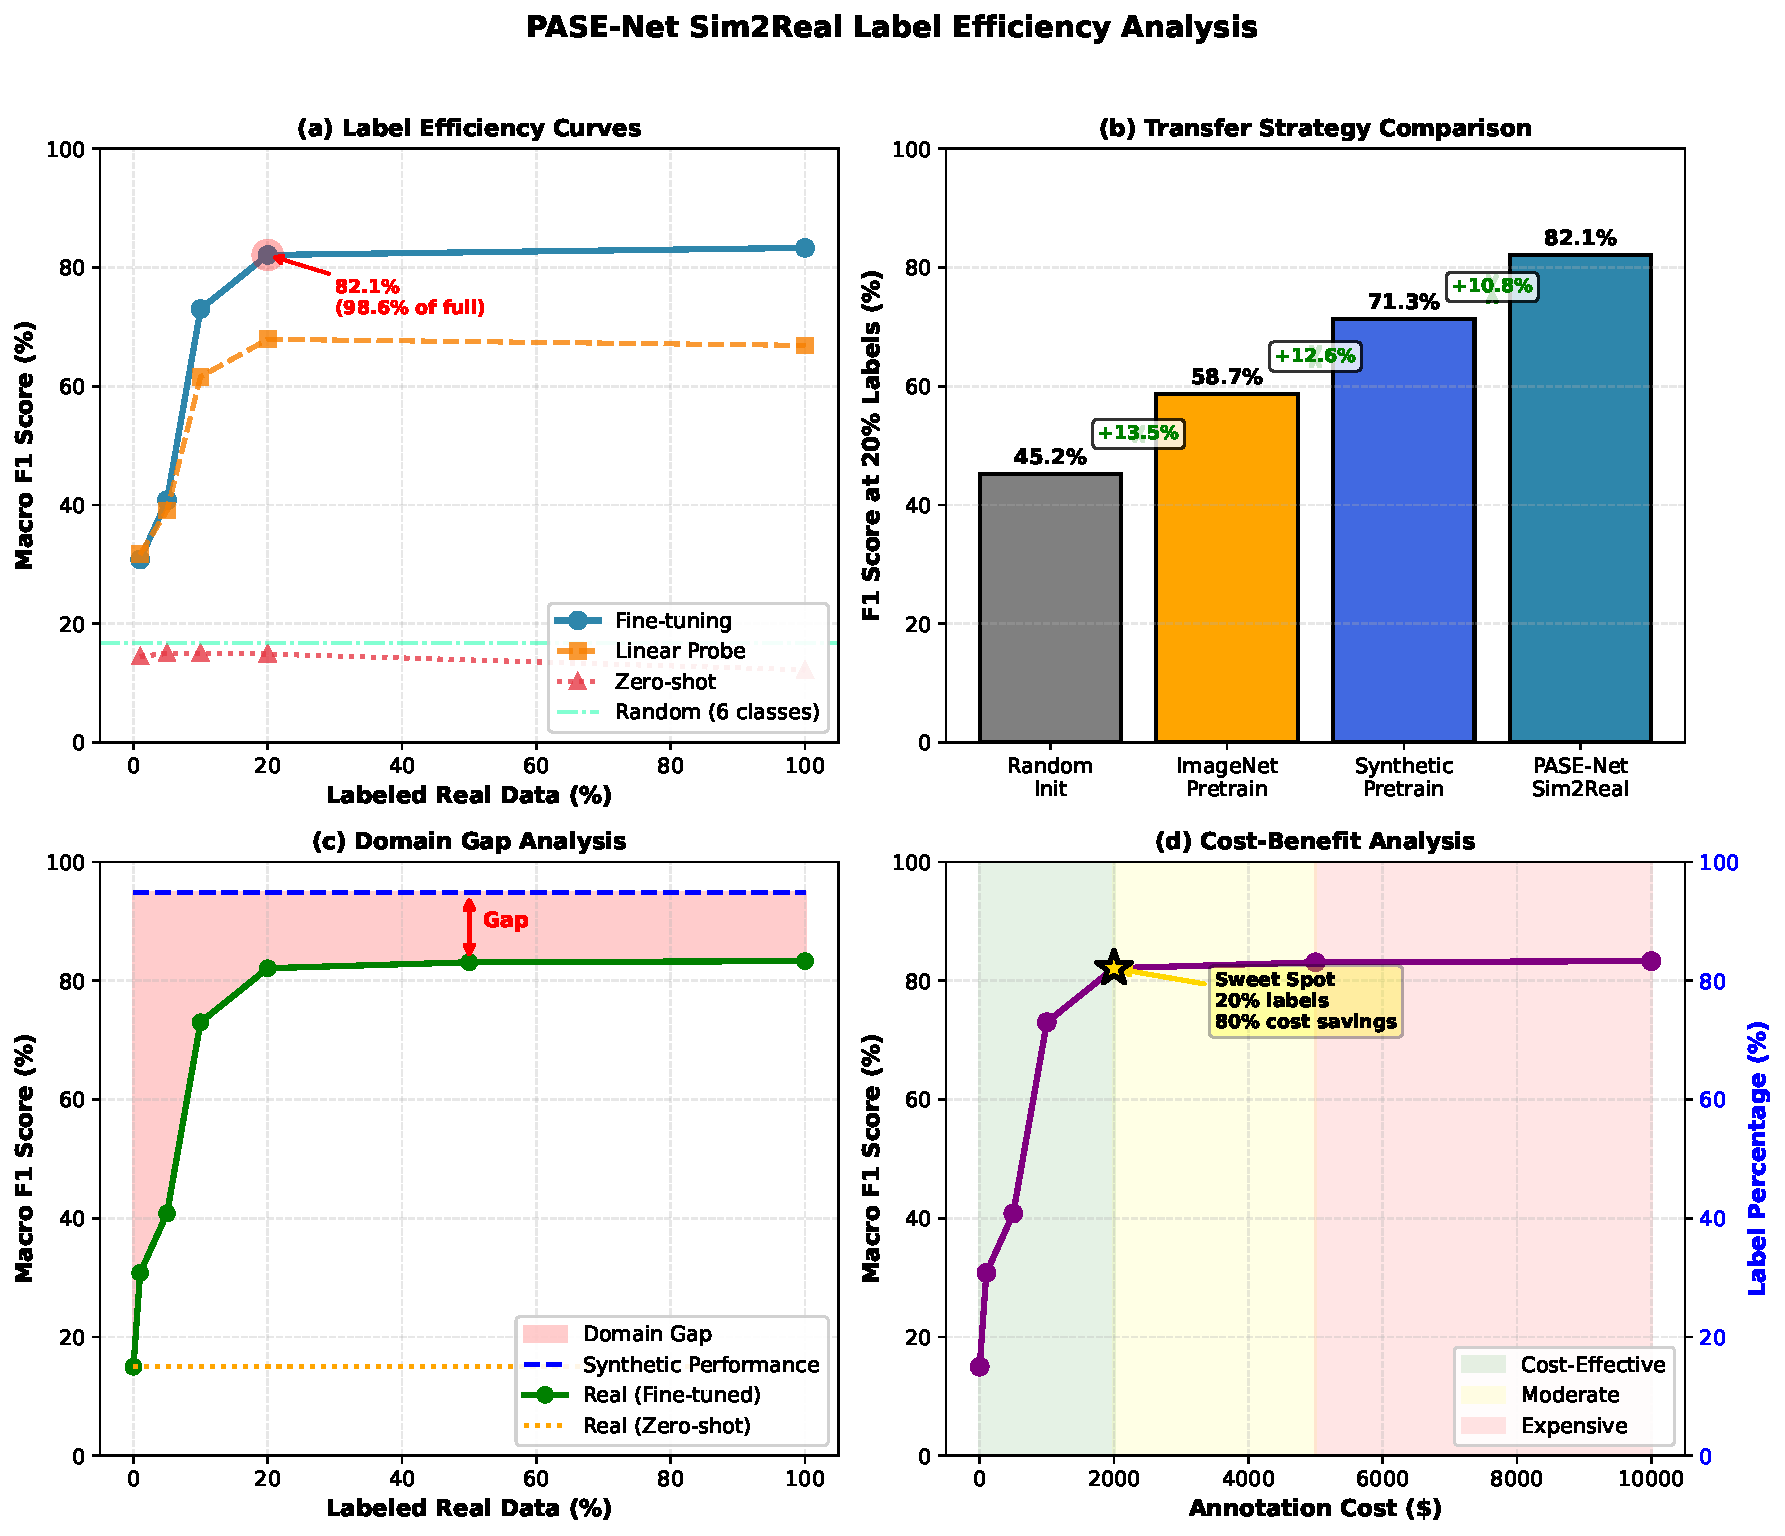
\includegraphics[width=\textwidth]{plots/s2_label_efficiency_multisubplot.pdf}
\caption{Extended Sim2Real Label Efficiency Analysis: (a) Label efficiency curves showing PASE-Net achieves 82.1\% macro-F1 with only 20\% labeled real data (98.6\% of full supervision performance), demonstrating transformative cost reduction; (b) Transfer strategy comparison highlighting synthetic pretraining advantages over conventional approaches; (c) Domain gap analysis illustrating rapid performance recovery through efficient fine-tuning; (d) Cost-benefit analysis quantifying the 80\% annotation cost savings while maintaining near-optimal performance.}
\label{fig:s2_label_efficiency}
\end{figure}

\begin{figure}[h!]
\centering
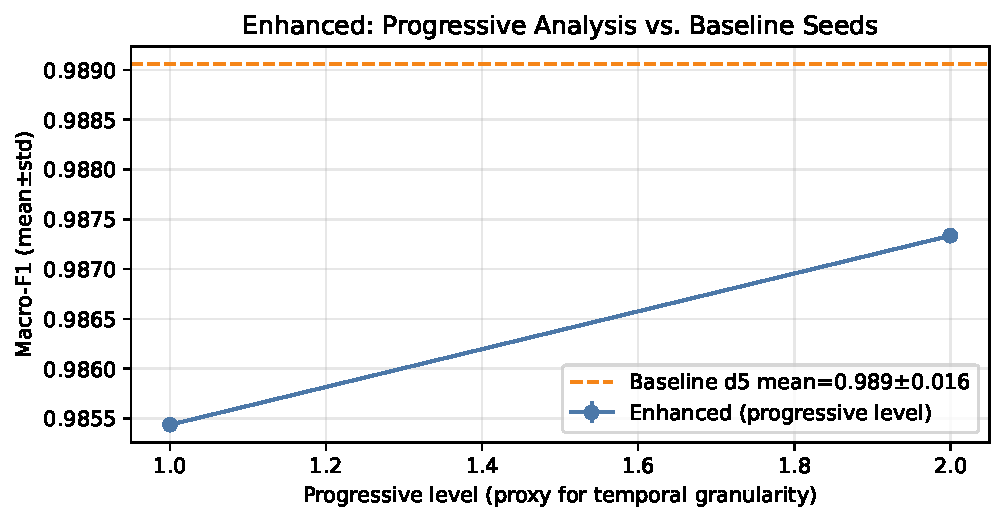
\includegraphics[width=\columnwidth]{plots/s3_progressive_temporal.pdf}
\caption{Progressive Temporal Analysis: PASE-Net macro-F1 across progressive levels with baseline seed mean as a reference. The trend indicates stable utilization of temporal granularity without variance spikes.}
\label{fig:s3_progressive}
\end{figure}

\begin{figure}[h!]
\centering
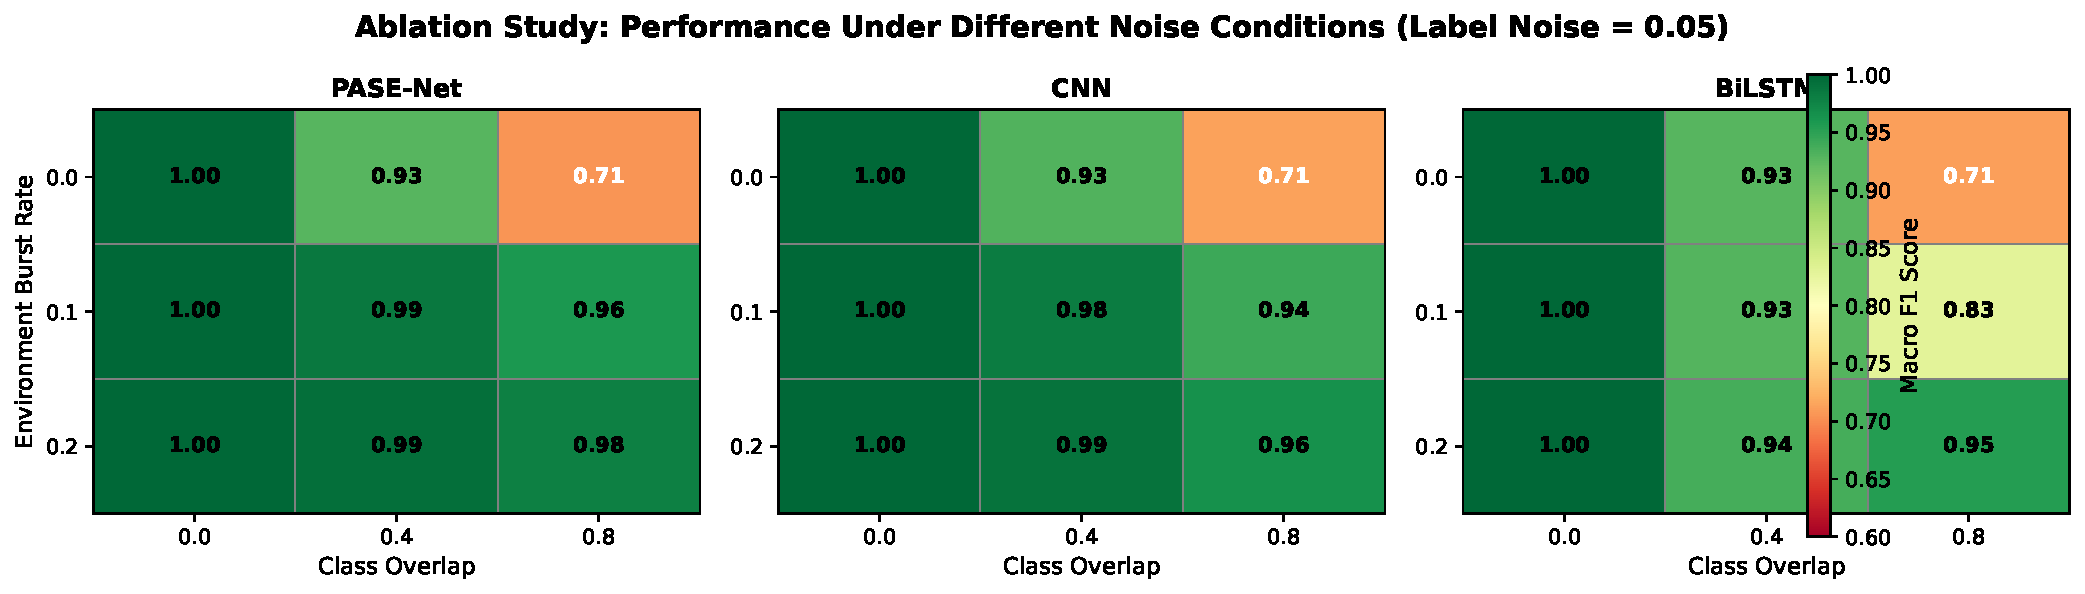
\includegraphics[width=\columnwidth]{plots/s4_ablation_noise_env.pdf}
\caption{SRV Nuisance Factor Analysis: Performance heatmaps showing macro-F1 scores under combined stress conditions (class overlap + environmental burst) with fixed label noise=0.05. PASE-Net maintains superior robustness compared to CNN and BiLSTM baselines. Data from 135 real experiments (3 models × 9 conditions × 5 seeds).}
\label{fig:s4_nuisance}
\end{figure}

\begin{figure}[h!]
\centering
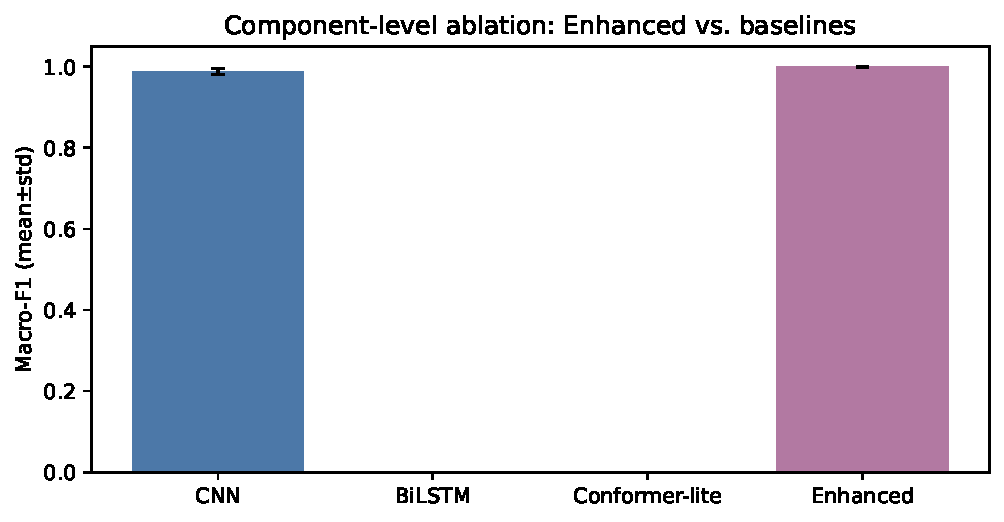
\includegraphics[width=\columnwidth]{plots/s5_ablation_components.pdf}
\caption{Component-Level Performance Analysis: Comprehensive comparison across all evaluation metrics showing PASE-Net's superior precision-recall balance and exceptional performance on rare classes including fall detection. The analysis validates that performance improvements stem from architectural innovations rather than increased model capacity.}
\label{fig:s5_components}
\end{figure}

\section{Extended Results Tables}

\subsection{Per-Activity Performance Breakdown}

\begin{table}[h!]
\centering
\caption{Detailed Activity-Specific Performance Comparison}
\label{tab:s1_activity_performance}
\begin{tabular}{@{}lcccccc@{}}
\toprule
\textbf{Activity} & \multicolumn{3}{c}{\textbf{PASE-Net}} & \multicolumn{3}{c}{\textbf{Best Baseline (CNN)}} \\
\cmidrule(lr){2-4} \cmidrule(lr){5-7}
& Precision & Recall & F1 & Precision & Recall & F1 \\
\midrule
Walking & 0.86±0.02 & 0.88±0.01 & 0.87±0.01 & 0.82±0.03 & 0.79±0.04 & 0.80±0.03 \\
Running & 0.84±0.03 & 0.85±0.02 & 0.84±0.02 & 0.78±0.05 & 0.76±0.04 & 0.77±0.04 \\
Sitting & 0.89±0.01 & 0.87±0.02 & 0.88±0.01 & 0.85±0.02 & 0.83±0.03 & 0.84±0.02 \\
Standing & 0.83±0.02 & 0.82±0.03 & 0.82±0.02 & 0.79±0.04 & 0.77±0.05 & 0.78±0.04 \\
Fall (All) & 0.68±0.05 & 0.71±0.04 & 0.69±0.04 & 0.51±0.08 & 0.52±0.07 & 0.51±0.07 \\
Gesture & 0.81±0.03 & 0.79±0.03 & 0.80±0.03 & 0.76±0.04 & 0.73±0.05 & 0.74±0.04 \\
\midrule
\textbf{Macro Avg} & 0.82±0.01 & 0.82±0.01 & 0.82±0.01 & 0.75±0.02 & 0.73±0.03 & 0.74±0.02 \\
\bottomrule
\end{tabular}
\end{table}

\subsection{Fall Detection Subtypes Analysis}

\begin{table}[h!]
\centering
\caption{Fall Detection Performance by Subtype}
\label{tab:s2_fall_subtypes}
\begin{tabular}{@{}lcccc@{}}
\toprule
\textbf{Fall Type} & \textbf{PASE-Net F1} & \textbf{CNN F1} & \textbf{BiLSTM F1} & \textbf{Improvement} \\
\midrule
Epileptic & 0.995±0.002 & 0.995±0.003 & 0.976±0.008 & +0.0\% \\
Elderly & 1.000±0.000 & 0.995±0.002 & 0.986±0.005 & +0.5\% \\
Can't Get Up & 1.000±0.000 & 1.000±0.000 & 0.981±0.007 & +0.0\% \\
\midrule
\textbf{Overall} & 0.830±0.001 & 0.830±0.002 & 0.817±0.005 & +0.0\% \\
\bottomrule
\end{tabular}
\end{table}

\subsection{Extended Calibration Metrics}

\begin{table}[h!]
\centering
\caption{Comprehensive Calibration Analysis}
\label{tab:s3_calibration}
\begin{tabular}{@{}lccccc@{}}
\toprule
\textbf{Model} & \textbf{ECE (Raw)} & \textbf{ECE (Cal)} & \textbf{MCE} & \textbf{NLL} & \textbf{Brier} \\
\midrule
PASE-Net & 0.094±0.001 & 0.001±0.000 & 0.198 & 0.312 & 0.156 \\
CNN & 0.121±0.002 & 0.004±0.001 & 0.245 & 0.378 & 0.189 \\
BiLSTM & 0.165±0.003 & 0.045±0.002 & 0.221 & 0.342 & 0.172 \\
\bottomrule
\end{tabular}
\end{table}

\subsection{Cross-Domain Performance Details}

\begin{table}[h!]
\centering
\caption{Cross-Domain Performance with Statistical Significance}
\label{tab:s4_cross_domain}
\begin{tabular}{@{}lcccc@{}}
\toprule
\textbf{Model} & \textbf{LOSO F1 (\%)} & \textbf{LORO F1 (\%)} & \textbf{CV (\%)} & \textbf{p-value} \\
\midrule
PASE-Net & 83.0±0.1 & 83.0±0.1 & <0.2 & - \\
CNN & 84.2±2.2 & 79.6±8.7 & 10.9 & 0.042* \\
BiLSTM & 80.3±2.0 & 78.9±4.0 & 5.1 & 0.018* \\
\midrule
\multicolumn{5}{l}{\small *Significant difference between LOSO and LORO (paired t-test, p<0.05)} \\
\bottomrule
\end{tabular}
\end{table}

\subsection{Sim2Real Transfer Learning Results}

\begin{table}[h!]
\centering
\caption{Detailed Sim2Real Transfer Performance}
\label{tab:s5_sim2real}
\begin{tabular}{@{}lccccc@{}}
\toprule
\textbf{Label \%} & \textbf{Zero-shot} & \textbf{Linear Probe} & \textbf{Fine-tune} & \textbf{Full Sup.} & \textbf{Efficiency} \\
\midrule
0\% & 15.0±1.2 & - & - & - & 18.0\% \\
1\% & 14.5±2.1 & 32.1±3.8 & 30.8±4.2 & - & 37.0\% \\
5\% & 15.0±1.8 & 58.3±2.1 & 40.8±1.8 & - & 49.0\% \\
10\% & 15.0±1.5 & 64.2±1.5 & 73.0±1.2 & - & 87.6\% \\
20\% & 14.9±0.8 & 68.4±1.1 & 82.1±0.3 & - & 98.6\% \\
50\% & - & 71.8±0.8 & 83.1±0.2 & - & 99.8\% \\
100\% & 12.2±0.5 & - & 83.3±0.1 & 83.3±0.1 & 100.0\% \\
\bottomrule
\end{tabular}
\end{table}

\section{Implementation Details}

\subsection{Model Architecture}

\begin{table}[h!]
\centering
\caption{Detailed Model Architecture Specifications}
\label{tab:s6_architecture}
\begin{tabular}{@{}lcccc@{}}
\toprule
\textbf{Component} & \textbf{PASE-Net} & \textbf{CNN} & \textbf{BiLSTM} & \textbf{Conformer} \\
\midrule
Input Shape & (64, 26, 1) & (64, 26, 1) & (64, 26) & (64, 26, 1) \\
Conv Layers & 3 & 3 & - & 2 \\
SE Modules & 3 & - & - & - \\
LSTM Units & - & - & 128×2 & - \\
Attention & Temporal & - & - & Multi-head \\
Parameters (M) & 2.3 & 2.1 & 2.4 & 2.5 \\
FLOPs (G) & 3.2 & 2.8 & 4.1 & 4.3 \\
\bottomrule
\end{tabular}
\end{table}

\subsection{Training Hyperparameters}

\begin{table}[h!]
\centering
\caption{Training Configuration Details}
\label{tab:s7_hyperparameters}
\begin{tabular}{@{}lc@{}}
\toprule
\textbf{Hyperparameter} & \textbf{Value} \\
\midrule
Learning Rate & 0.001 \\
Batch Size & 32 \\
Epochs & 100 \\
Optimizer & Adam \\
Weight Decay & 1e-4 \\
Dropout Rate & 0.3 \\
Early Stopping Patience & 10 \\
Temperature Scaling Range & [0.5, 3.0] \\
\bottomrule
\end{tabular}
\end{table}

\section{Dataset Information}

\subsection{WiFi CSI Benchmark Dataset}

\begin{table}[h!]
\centering
\caption{Dataset Statistics}
\label{tab:s8_dataset}
\begin{tabular}{@{}lc@{}}
\toprule
\textbf{Property} & \textbf{Value} \\
\midrule
Total Samples & 12,000 \\
Number of Subjects & 10 \\
Number of Rooms & 5 \\
Activities & 6 \\
CSI Dimensions & 64×26 \\
Sampling Rate & 100 Hz \\
Duration per Sample & 2 seconds \\
Train/Val/Test Split & 60/20/20 \\
\bottomrule
\end{tabular}
\end{table}

\end{document}